\documentclass{beamer}


\usepackage{etex}
\usepackage{pgffor}
\usepackage[utf8]{inputenc}
%\reserveinserts{28}

\usepackage[backend=biber, citestyle=authoryear, maxcitenames=2, maxbibnames=20]{biblatex}
\bibliography{../biblio.bib}

\usepackage{amsmath,amssymb,amsthm,dsfont}
\usepackage{amsfonts}
\usepackage{mathtools}
\usepackage{color}
\usepackage{esint}
\usepackage{stmaryrd}
\usepackage{tabularx}
\usepackage{multirow}
\usepackage[squaren]{SIunits}
\usepackage{graphicx}
\usepackage{subfig}
\usepackage{diagbox}
\usepackage{pdfpages}
\usepackage{dsfont}
\usepackage{xcolor}
\usepackage{soul}
\usepackage[linesnumbered,ruled,vlined]{algorithm2e}
\usepackage{algorithmic}

\usepackage{hyperref}
\usepackage{multimedia}
\usepackage{array}
\usepackage{multirow}
\usepackage{booktabs}
\usepackage{eso-pic}
\usepackage{monster2e}
\usepackage{tikz}
\usepackage{svg}
\usepackage{layout}
\usepackage{xcolor}
\usepackage{fancybox}
\usepackage{setspace}
\usepackage{bbding}
\usepackage{calc}
\usepackage{multicol}
\usepackage[absolute,showboxes,overlay]{textpos}
\usetikzlibrary{calc,fadings,mindmap,trees,arrows,calc,tikzmark,shapes}
\usepackage[flushleft]{threeparttable}

\TPshowboxesfalse
\textblockorigin{0mm}{0mm}
\newcommand{\mathcolorbox}[2]{\colorbox{#1}{$\displaystyle #2$}}

% Icons
\newcommand{\vcenteredinclude}[2]{\begingroup
\setbox0=\hbox{\includesvg[scale=#2]{#1}}%
\parbox{\wd0}{\box0}\endgroup}


% Change margins for slides
\newenvironment{changemargin}[2]{% 
	\begin{list}{}{% 
			\setlength{\topsep}{0pt}% 
			\setlength{\leftmargin}{#1}% 
			\setlength{\rightmargin}{#2}% 
			\setlength{\listparindent}{\parindent}% 
			\setlength{\itemindent}{\parindent}% 
			\setlength{\parsep}{\parskip}% 
		}% 
		\item[]}{\end{list}} 


% Input

% Colors for slides
\definecolor{rouge1}{RGB}{226,0,38}  % red P
\definecolor{orange1}{RGB}{243,154,38}  % orange P
\definecolor{jaune}{RGB}{254,205,27}  % jaune P
\definecolor{blanc}{RGB}{255,255,255} % blanc P

\definecolor{rouge2}{RGB}{230,68,57}  % red S
\definecolor{orange2}{RGB}{236,117,40}  % orange S
\definecolor{taupe}{RGB}{134,113,127} % taupe S
\definecolor{gris}{RGB}{91,94,111} % gris S
\definecolor{bleu1}{RGB}{38,109,131} % bleu S
\definecolor{bleu2}{RGB}{28,50,114} % bleu S
\definecolor{vert1}{RGB}{133,146,66} % vert S
\definecolor{vert3}{RGB}{20,200,66} % vert S
\definecolor{vert2}{RGB}{157,193,7} % vert S
\definecolor{vertsolarized}{RGB}{211,233,219} % vert S
\definecolor{darkyellow}{RGB}{233,165,0}  % orange S
\definecolor{lightgray}{rgb}{0.9,0.9,0.9}
\definecolor{darkgray}{rgb}{0.6,0.6,0.6}

\newcommand{\incarrow}{{
\includegraphics[height=0.7\baselineskip]{./img/arrow_list}}}


% Highlights for slides
\newcommand{\rcol}[1]{\textcolor{red}{\textit{#1}}}
%\newcommand{\eqrcol}[1]{\textcolor{red}{#1}}
%\newcommand{\eqrcolb}[1]{\textcolor{red}{\boldsymbol{#1}}}
\newcommand{\gcol}[1]{\textcolor{vert3}{\textit{#1}}}
%\newcommand{\eqgcol}[1]{\textcolor{vert3}{#1}}
%\newcommand{\eqgcolb}[1]{\textcolor{vert3}{\boldsymbol{#1}}}
\newcommand{\blcol}[1]{\textcolor{blue}{\textit{#1}}}
%\newcommand{\eqbcol}[1]{\textcolor{blue}{#1}}
%\newcommand{\eqbcolb}[1]{\textcolor{blue}{\boldsymbol{#1}}}
\newcommand{\ycol}[1]{\textcolor{darkyellow}{\textit{#1}}}
\newcommand{\eqycol}[1]{\textcolor{darkyellow}{#1}}

\newcommand{\rcolbm}[1]{$\textcolor{red}{\boldsymbol{#1}}$}
\newcommand{\rcolb}[1]{\textcolor{red}{\textit{\textbf{#1}}}}
\newcommand{\gcolb}[1]{\textcolor{vert3}{\textit{\textbf{#1}}}}
\newcommand{\bcolb}[1]{\textcolor{blue}{\textit{\textbf{#1}}}}
\newcommand{\ycolb}[1]{\textcolor{darkyellow}{\textit{\textbf{#1}}}}

% Colored boxes
\newcounter{ColoredBoxesCounter}
\newcommand{\highlightnew}[3][(0.0,-0.1)(-0.0,0.3)]{
\hfsetfillcolor{#2!20}
\hfsetbordercolor{#2!80}
\tikzmarkin{\theColoredBoxesCounter}#1
#3
\tikzmarkend{\theColoredBoxesCounter}
\stepcounter{ColoredBoxesCounter}
}

\newcommand{\highlight}[2][yellow]{\mathchoice%
{\colorbox{#1}{$\displaystyle#2$}}%
{\colorbox{#1}{$\textstyle#2$}}%
{\colorbox{#1}{$\scriptstyle#2$}}%
{\colorbox{#1}{$\scriptscriptstyle#2$}}}%

\newcommand{\eqrcol}[1]{\highlight[red!20]{#1}}
\newcommand{\eqrcolb}[1]{\highlight[red!20]{\boldsymbol{#1}}}
\newcommand{\eqgcol}[1]{\highlight[vert3!20]{#1}}
\newcommand{\eqgcolb}[1]{\highlight[vert3!20]{\boldsymbol{#1}}}
\newcommand{\eqbcol}[1]{\highlight[blue!20]{#1}}
\newcommand{\eqbcolb}[1]{\highlight[blue!20]{\boldsymbol{#1}}}

\colorlet{redp}{red!20} % vert S
\colorlet{greenp}{vert3!20} % vert S
\colorlet{bluep}{blue!20} % vert S
\colorlet{yellowp}{yellow!20} % vert S

\renewcommand{\hl}[3][\fboxsep1pt]{{#1\colorbox{#2}{#3}}}%

\newcommand{\hlr}[1]{\hl{redp}{#1}}
\newcommand{\hlg}[1]{\hl{greenp}{#1}}
\newcommand{\hlb}[1]{\hl{bluep}{#1}}
\newcommand{\hly}[1]{\hl{yellowp}{#1}}

\newcommand{\hler}[1]{\hl[\fboxsep0pt]{redp}{$\displaystyle {#1}$}}
\newcommand{\hleg}[1]{\hl[\fboxsep0pt]{greenp}{$\displaystyle {#1}$}}
\newcommand{\hleb}[1]{\hl[\fboxsep0pt]{bluep}{$\displaystyle {#1}$}}

\newcommand{\hlbr}[1]{\hl[\fboxsep0pt]{redp}{$\displaystyle \mathbf{#1}$}}
\newcommand{\hlbg}[1]{\hl[\fboxsep0pt]{greenp}{$\displaystyle \mathbf{#1}$}}
\newcommand{\hlbb}[1]{\hl[\fboxsep0pt]{bluep}{$\displaystyle \mathbf{#1}$}}

\newcommand{\vph}{\vphantom{A_A^A}}

% Box for algorithms
\newlength{\minipagewidth}
\newlength{\minipagewidthx}
\setlength{\minipagewidth}{\columnwidth}
\setlength{\minipagewidthx}{\columnwidth}
\setlength{\fboxsep}{0.1mm}
\addtolength{\minipagewidth}{-\fboxrule}
\addtolength{\minipagewidth}{-\fboxrule}
\addtolength{\minipagewidth}{-\fboxsep}
\addtolength{\minipagewidth}{-\fboxsep}
\addtolength{\minipagewidthx}{+\fboxsep}
\newcommand{\bookbox}[1]{\small
\par\medskip\noindent
\framebox[\columnwidth]{
\begin{minipage}{\minipagewidth} {#1} \end{minipage} } \par\medskip }

\newcommand{\bookboxx}[1]{
\par\medskip\noindent
\framebox[\columnwidth]{
\begin{minipage}[t]{0.98\columnwidth} {\par\smallskip#1\par\smallskip} \end{minipage} } \par\medskip }


\usepackage{array}
\newcolumntype{L}[1]{>{\raggedright\let\newline\\\arraybackslash\hspace{-3.1cm}}m{#1}}
\newcolumntype{C}[1]{>{\centering\let\newline\\\arraybackslash\hspace{135pt}}m{#1}}
\newcolumntype{R}[1]{>{\raggedleft\let\newline\\\arraybackslash\hspace{-10pt}}m{#1}}

\newenvironment{myfont}{\fontfamily{kurier}\selectfont}{\par}
\newenvironment{myfont2}{\fontfamily{epigrafica}\selectfont}{\par}

% Border color of content boxes
\definecolor{bordercol}{RGB}{0,0,0}  %black
% Background color for the header in the content boxes (left side)
\definecolor{headercol1}{RGB}{200,0,0}        %red:RGB {200,0,0} 
% Background color for the header in the content boxes (right side) 
\definecolor{headercol2}{rgb}{1.0,0.49,0.0}        %orange:rgb {1.0,0.49,0.0}
% Text color for the header text in the content boxes
\definecolor{headerfontcol}{rgb}{1,1,1}  %white
% Background color for the content in the boxes
\definecolor{boxcolor}{rgb}{1,1,1} 

\definecolor{lightblue}{rgb}{0.145,0.6666,1}

\newsavebox\CBox
\newcommand\hcancel[2][0.5pt]{%
  \ifmmode\sbox\CBox{$#2$}\else\sbox\CBox{#2}\fi%
  \makebox[0pt][l]{\usebox\CBox}%  
  \rule[0.3\ht\CBox-#1/2]{\wd\CBox}{#1}}



%%%%%%%%%%%%%%%%%%%%%%%%%%%%
% Paper dependent stuff    %
%%%%%%%%%%%%%%%%%%%%%%%%%%%%

\newcommand{\Tau}{\mathcal{T}}
\newcommand{\LL}{\mathcal{L}}
\newcommand{\dquad}{d_\texttt{QUAD}}
\newcommand{\dber}{d_\texttt{BER}}
\newcommand{\OLOP}{\texttt{OLOP}\xspace}
\newcommand{\ODP}{\texttt{ODP}\xspace}
\newcommand{\KLOLOP}{\texttt{KL-OLOP}\xspace}
\newcommand{\klOLOP}{\texttt{kl-OLOP}\xspace}


%%%%%%%%%%%%%%%%%%%%%%%%%%%%
% Aesthetics               %
% over-underline, hat, bold%
%%%%%%%%%%%%%%%%%%%%%%%%%%%%

%%% miso
\newcommand{\eps}{\varepsilon}
\newcommand{\vareps}{\varepsilon}
\renewcommand{\epsilon}{\varepsilon}
%\renewcommand{\hat}{\widehat}
\renewcommand{\tilde}{\widetilde}
\renewcommand{\bar}{\overline}

\newcommand*{\MyDef}{\mathrm{\tiny def}}
\newcommand*{\eqdefU}{\ensuremath{\mathop{\overset{\MyDef}{=}}}}% Unscaled version
%\newcommand*{\eqdef}{\mathop{\overset{\MyDef}{\resizebox{\widthof{\eqdefU}}{\heightof{=}}{=}}}}


\def\:#1{\protect \ifmmode {\mathbf{#1}} \else {\textbf{#1}} \fi}
\newcommand{\CommaBin}{\mathbin{\raisebox{0.5ex}{,}}}

\newcommand{\wt}[1]{\widetilde{#1}}
\newcommand{\wh}[1]{\widehat{#1}}
\newcommand{\wo}[1]{\overline{#1}}
\newcommand{\wb}[1]{\overline{#1}}

% bf and bm missing due to conflict!!
\newcommand{\bsym}[1]{\mathbf{#1}}
\newcommand{\bzero}{\mathbf{0}}
\newcommand{\ba}{\mathbf{a}}
\newcommand{\bb}{\mathbf{b}}
\newcommand{\bc}{\mathbf{c}}
\newcommand{\bd}{\mathbf{d}}
\newcommand{\be}{\mathbf{e}}
\newcommand{\bg}{\mathbf{g}}
\newcommand{\bh}{\mathbf{h}}
\newcommand{\bi}{\mathbf{i}}
\newcommand{\bj}{\mathbf{j}}
\newcommand{\bk}{\mathbf{k}}
\newcommand{\bl}{\mathbf{l}}
\newcommand{\bn}{\mathbf{n}}
\newcommand{\bo}{\mathbf{o}}
\newcommand{\bp}{\mathbf{p}}
\newcommand{\bq}{\mathbf{q}}
\newcommand{\br}{\mathbf{r}}
\newcommand{\bs}{\mathbf{s}}
\newcommand{\bt}{\mathbf{t}}
\newcommand{\bu}{\mathbf{u}}
\newcommand{\bv}{\mathbf{v}}
\newcommand{\bw}{\mathbf{w}}
\newcommand{\bx}{\mathbf{x}}
\newcommand{\by}{\mathbf{y}}
\newcommand{\bz}{\mathbf{z}}

\newcommand{\bA}{\mathbf{A}}
\newcommand{\bB}{\mathbf{B}}
\newcommand{\bC}{\mathbf{C}}
\newcommand{\bD}{\mathbf{D}}
\newcommand{\bE}{\mathbf{E}}
\newcommand{\bF}{\mathbf{F}}
\newcommand{\bG}{\mathbf{G}}
\newcommand{\bH}{\mathbf{H}}
\newcommand{\bI}{\mathbf{I}}
\newcommand{\bJ}{\mathbf{J}}
\newcommand{\bK}{\mathbf{K}}
\newcommand{\bL}{\mathbf{L}}
\newcommand{\bM}{\mathbf{M}}
\newcommand{\bN}{\mathbf{N}}
\newcommand{\bO}{\mathbf{O}}
\newcommand{\bP}{\mathbf{P}}
\newcommand{\bQ}{\mathbf{Q}}
\newcommand{\bR}{\mathbf{R}}
\newcommand{\bS}{\mathbf{S}}
\newcommand{\bT}{\mathbf{T}}
\newcommand{\bU}{\mathbf{U}}
\newcommand{\bV}{\mathbf{V}}
\newcommand{\bW}{\mathbf{W}}
\newcommand{\bX}{\mathbf{X}}
\newcommand{\bY}{\mathbf{Y}}
\newcommand{\bZ}{\mathbf{Z}}

% calligraphic
\newcommand{\cf}{\mathcal{f}}
\newcommand{\cA}{\mathcal{A}}
\newcommand{\cB}{\mathcal{B}}
\newcommand{\cC}{\mathcal{C}}
\newcommand{\cD}{\mathcal{D}}
\newcommand{\cE}{\mathcal{E}}
\newcommand{\cF}{\mathcal{F}}
\newcommand{\cG}{\mathcal{G}}
\newcommand{\cH}{\mathcal{H}}
\newcommand{\cI}{\mathcal{I}}
\newcommand{\cJ}{\mathcal{J}}
\newcommand{\cK}{\mathcal{K}}
\newcommand{\cL}{\mathcal{L}}
\newcommand{\cM}{\mathcal{M}}
\newcommand{\cN}{\mathcal{N}}
\newcommand{\cO}{\mathcal{O}}
\newcommand{\cP}{\mathcal{P}}
\newcommand{\cQ}{\mathcal{Q}}
\newcommand{\cR}{\mathcal{R}}
\newcommand{\cS}{\mathcal{S}}
\newcommand{\cT}{\mathcal{T}}
\newcommand{\cU}{\mathcal{U}}
\newcommand{\cV}{\mathcal{V}}
\newcommand{\cW}{\mathcal{W}}
\newcommand{\cX}{\mathcal{X}}
\newcommand{\cY}{\mathcal{Y}}
\newcommand{\cZ}{\mathcal{Z}}

%%%%%%%%%%%%%%%%%%%%%%%%%%%%
% Math jargon              %
%%%%%%%%%%%%%%%%%%%%%%%%%%%%
\newcommand{\wrt}{w.r.t.\xspace}
\newcommand{\defeq}{\stackrel{\mathclap{\normalfont\mbox{\tiny def}}}{=}}
\newcommand{\maxund}[1]{\max\limits_{#1}}
\newcommand{\supund}[1]{\text{sup}\limits_{#1}}
\newcommand{\minund}[1]{\min\limits_{#1}}
\renewcommand{\epsilon}{\varepsilon}
\newcommand{\bigotime}{\mathcal{O}}


\DeclareMathOperator*{\argmin}{arg\,min} 
\DeclareMathOperator*{\argmax}{arg\,max} 
\DeclareMathOperator*{\cupdot}{\mathbin{\mathaccent\cdot\cup}}
\newcommand{\eqdef}{\buildrel \text{def}\over =}

%%%%%%%%%%%%%%%%%%%%%%%%%%%%
% Matrix operators         %
%%%%%%%%%%%%%%%%%%%%%%%%%%%%
\newcommand{\transpose}{^\mathsf{\scriptscriptstyle T}}
\newcommand{\transp}{\mathsf{\scriptscriptstyle T}}

%%%%%%%%%%%%%%%%%%%%%%%%%%%%
% Statistic operators      %
%%%%%%%%%%%%%%%%%%%%%%%%%%%%
\newcommand{\probability}[1]{\mathbb{P}\left(#1\right)}
\newcommand{\probdist}{Pr}
\DeclareMathOperator*{\expectedvalue}{\mathbb{E}}
\DeclareMathOperator*{\variance}{\text{Var}}
\newcommand{\expectedvalueover}[1]{\expectedvalue\limits_{#1}}
\newcommand{\condbar}{\;\middle|\;}
\newcommand{\gaussdistr}{\mathcal{N}}
\newcommand{\uniformdistr}{\mathcal{U}}
\newcommand{\bernoullidist}{\mathcal{B}}

%%%%%%%%%%%%%%%%%%%%%%%%%%%%
% Algebraic Sets           %
%%%%%%%%%%%%%%%%%%%%%%%%%%%%
\newcommand{\Real}{\mathbb{R}}
\newcommand{\Natural}{\mathbb{N}}
\newcommand{\statespace}{\mathcal{X}}
\newcommand{\funcspace}{\mathcal{F}}
\newcommand{\dynaspace}{\mathcal{T}}


% \newtheorem{theorem}{Theorem}
% \newtheorem{definition}{Definition}
% \newtheorem{lemma}{Lemma}
\newtheorem{proposition}{Proposition}
\newtheorem{assumption}{Assumption}
\newtheorem{remark}{Remark}
\newtheorem{property}{Property}
\newtheorem{proposition}{Proposition}
\newtheorem{assumption}{Assumption}
\newtheorem{remark}{Remark}
\newtheorem{property}{Property}

% Style

\TPshowboxesfalse
\textblockorigin{0mm}{0mm}

\setbeamertemplate{footline}{% 
  \hfill% 
  \usebeamercolor[fg]{page number in head/foot}% 
  \usebeamerfont{page number in head/foot}% 
  \insertframenumber%
  %\,/\,\inserttotalframenumber
  \kern1em\vskip2pt% 
}
\beamertemplatenavigationsymbolsempty
\setbeamertemplate{navigation symbols}{}
%\setbeamertemplate{blocks}[rounded]
%\setbeamercolor{block title}{bg=bleu2,fg=white}%bg=background, fg= foreground
%\setbeamercolor{block body}{bg=lightgray}%bg=background, fg= foreground
\renewcommand{\sfdefault}{lmss}
\sffamily
\setbeamersize{text margin left=1cm,text margin right=1cm}


\author[shortname]{
Edouard Leurent \inst{1}, \inst{2} \and 
Odalric-Ambrym Maillard\inst{1}}
\institute[shortinst]{\inst{1} Inria SequeL.\and %
                      \inst{2} Renault Group.}

\title[]{Practical Open-Loop Optimistic Planning}
\date{}
\begin{document}
	
\setbeamertemplate{background canvas}[vertical shading][top=bleu2,middle=bleu2,bottom=bleu1]
\setbeamertemplate{footline}{\hspace{5em} \textcolor{white} {\null \hfill
		\scriptsize Würzburg, September 2019}\hspace{2em}\null \vspace*{3pt}}
	
\begin{frame}
\begin{textblock*}{40mm}[0,0](10mm,0mm)
	
\includegraphics[width=3.4cm]{inria/logobleu2}
\end{textblock*}
\begin{textblock*}{40mm}[0,0](14mm,3mm)
	
\includegraphics[width=2.6cm]{inria/renault_group}
\end{textblock*}

\begin{textblock*}{11.8cm}(4mm,40mm)
	\vspace{.3cm}
	\textcolor{white} {
		\Large \textbf{\hspace{0.5em}Practical Open-Loop Optimistic Planning}\\
		{\small %
			\vspace{1cm}
			\hspace{1.5em}\large\textbf{Edouard Leurent$^{1,2}$, Odalric-Ambrym Maillard$^1$}\\
			\hspace{2.5em}${}^1$ SequeL, Inria Lille -- Nord Europe\\
			\hspace{2.5em}${}^2$ Renault Group\\
	}}
\end{textblock*}

\begin{textblock*}{40mm}[0,0](10mm,76mm)
	\begin{picture}(5,80)
	\put(0,20){
\includegraphics[width=3.8cm,height=1.5cm]{inria/logobasbleuV1}}
	\put(13,35){
		\footnotesize \textcolor{bleu2}{ECML PKDD 2019}
	}
	\end{picture}
\end{textblock*}

\vspace*{-4pt}
\end{frame}

\setbeamertemplate{background canvas}[vertical shading][top=blanc, middle=blanc,bottom=blanc]
\setbeamercolor{footlinecolor}{fg=blanc,bg=bleu2}
\setbeamertemplate{footline}
{
\begin{beamercolorbox}[wd=1\paperwidth,ht=15.5pt]{footlinecolor}
		\hspace{3mm}
		
\includegraphics[width=14mm]{inria/logobastrans}
		\hspace{.4cm}
		\raisebox{3.2ex}
		{\scriptsize Practical Open-Loop Optimistic Planning}\hfill
		\raisebox{3.2ex}
		{Würzburg - \insertframenumber/\inserttotalframenumber \hspace{5mm}
			\null }
\end{beamercolorbox}
}

\begin{frame}{Motivation | Sequential Decision Making}

\begin{block}{Markov Decision Processes}
\begin{enumerate}
    \item Observe state $s\in S$;
    \item Pick a \hlb{discrete} action $a\in A$;
    \item Transition to a next state $s'\sim \hler{\probability{s'|s,a}}$;
    \item Receive a \hlb{bounded} reward $r\in[0, 1]$ drawn from $\hler{\probability{r|s, a}}$.
\end{enumerate}
\begin{center}
    Objective: maximise \hlg{V = $\expectedvalue \left[\sum_{t=0}^\infty \gamma^t r_t \right]$}
\end{center}
\end{block}

\end{frame}

\begin{frame}{Motivation | How to solve MDPs?}

% \begin{block}{Dynamic Programming}
% \begin{itemize}
%     \item The transition and reward kernels $\probability{s',r|s,a}$ are \hlg{known};
%     \item[\incarrow] The problem reduces to solving a \hlg{linear program}.
% \end{itemize}
% \end{block}

\begin{exampleblock}{Online \emph{Planning}}
\begin{itemize}
    \item the transition kernel and reward kernel are \hlr{unknown}
    \item we have access to a \hlg{generative model}: 
    \begin{itemize}
        \item[\incarrow] yields samples of $s', r \sim \probability{s',r|s,a}$ when queried
    \end{itemize}
    \item \hlr{fixed budget}: the model can only be queried $n$ times
\end{itemize}
\begin{center}
Objective: \hlg{minimize} $\expectedvalue \underbrace{r_n = V^* - V(n)}_{\text{Simple Regret}}$
\end{center}
\end{exampleblock}
\end{frame}


\begin{frame}{Optimistic Planning}
    
    
    \begin{alertblock}{Previously: Combinatorial Search}
    \begin{itemize}
        \item Branch pruning and heuristic utility functions
    \end{itemize}
    \end{alertblock}
    
    \begin{exampleblock}{Optimism in the Face of Uncertainty}
    Given a set of decisions $a\in A$ with uncertain outcomes $\nu_a$, pick the one with the \hlg{highest upper-confidence bound}.
    
    \begin{itemize}
        \item Either you performed well;
        \item or you learned something.
    \end{itemize}
    \end{exampleblock}
    
    
    \begin{block}{Instances}
    \begin{itemize}
        \item Monte-carlo tree search [\cite{Coulom2006}]: for playing Go
        \item Reframed in the bandit setting as \texttt{UCT} [\cite{Kocsis2006}]
        \item Asymptotic analysis but no finite time guarantee.
    \end{itemize}
    \end{block}
\end{frame}


\begin{frame}{Failing cases of \texttt{UCT}}
    It was analysed in [\cite{Coquelin2007}]
    \begin{center}
    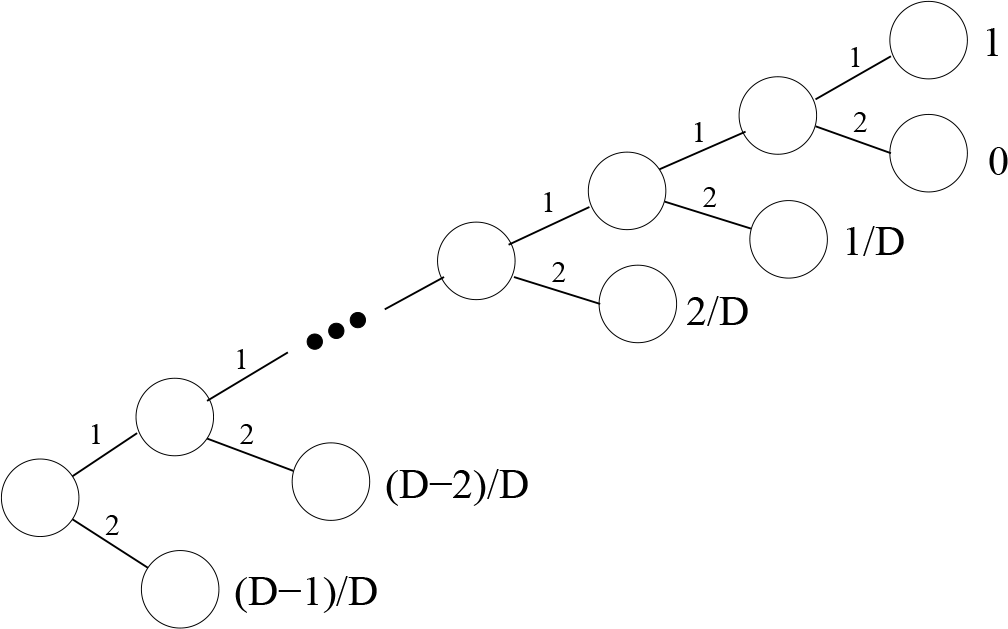
\includegraphics[width=0.8\textwidth]{img/uct_fail}
    \end{center}
    The sample complexity of is lower-bounded by \hlr{$O(\exp(\exp(D)))$}.
\end{frame}

\begin{frame}{Failing cases of \texttt{UCT}}
    Not just a theoretical counter-example.
    \begin{center}
    
\includegraphics[width=0.8\textwidth]{img/uct_trap}\\
    \bigskip
    \includesvg[width=0.5\textwidth]{img/uct_fail_hw}
    \end{center}
\end{frame}

\begin{frame}{Can we get better guarantees?}
    \begin{block}{\OPD: Optimistic Planning for Deterministic systems}
    \begin{itemize}
        \item Introduced by [\cite{Hren2008}]
        \item Another \hlg{optimistic} algorithm
        \item Only for \hlr{deterministic} MDPs
    \end{itemize}
    \end{block}
    \begin{theorem}[\OPD sample complexity]
    \begin{equation*}
    \expectedvalue r_n = 
      \cO\left(n^{-\frac{\log 1/\gamma}{\log \kappa}}\right), \text{if}\ \kappa > 1 
    \end{equation*}
    \end{theorem}
\begin{block}{\OLOP: Open-Loop Optimistic Planning}
    \begin{itemize}
        \item Introduced by [\cite{Bubeck2010}]
        \item Extends \OPD to the \hlg{stochastic} setting
        \item Only considers \hlr{open-loop} policies, i.e. sequences of actions
    \end{itemize}
    \end{block}
\end{frame}

% \begin{frame}{A Benchmark of Planning Algorithms}
%     \small
%     \begin{threeparttable}
%     \centering
%     \begin{tabular}{cccc}
%     \toprule
%         Algorithm & Complexity & Does it run? & Does it work?\\
%         \midrule
%         \texttt{MCTS} & ? & \hlg{YES} & ?\\
%         \texttt{SparseSampling}\tnote{1} & $(1/\epsilon)^{\log 1/\epsilon}$ & \hlg{YES} & \hlr{NO} \\
%         \texttt{UCT} & $\exp(\exp(D))$ & \hlg{YES} & \hly{KIND OF} \\
%         \texttt{OPD}\tnote{2} & $n^{-\frac{\log1/\gamma}{\log \kappa}}$ & \hlg{YES} & \hlg{YES} \\
%         \OLOP & $n^{-\min(\frac{1}{2}, \frac{\log1/\gamma}{\log \kappa})}$ & \hly{KIND OF} & \hlr{NO} \\
%         \texttt{ST0P}\tnote{1} & $(1/\epsilon)^{2+\frac{\log \kappa'}{\log1/\gamma}+o(1)}$ & \hlr{NO} & ? (\hlr{NO})\\
%         \texttt{TrailBlazer}\tnote{1} & $(1/\epsilon)^{\frac{\log N\kappa}{\log1/\gamma}}(\log\frac{1}{\delta\epsilon})^\alpha$ & \hlg{YES} & \hlr{NO}\\
%         \texttt{PlatYPOOs}\tnote{2} & $\leq$ \OLOP & \hlg{YES} & \hlg{YES}\\
%         \bottomrule
%     \end{tabular}
    
%     \begin{tablenotes}
%     \item[1] In the PAC framework. 
%     \item[2] With deterministic dynamics
%     \end{tablenotes}
%     \end{threeparttable}
% \end{frame}

\begin{frame}{The idea behind \OLOP}
\begin{center}
\includesvg[width=0.8\textwidth]{img/olop-explain}
\end{center}
% \begin{center}
% \scalebox{0.7}{
% \begin{algorithm}[H]
% \DontPrintSemicolon
% \footnotesize
% \For{each episode $m = 1, \cdots, M$}{
% Compute $U_a(m-1)$ from \eqref{eq:Ua} for all $a\in\mathcal{T}$\;
% Compute $B_a(m-1)$ from \eqref{eq:Ba} for all $a\in A^L$\;\label{alg:b_values_compute}
% Sample a sequence with highest B-value: $a^m \in \argmax_{a\in A^L} B_a(m-1)$.\;
% }
% \Return the most played sequence $a(n) \in \argmax_{a\in A^L} T_a(M)$
% \caption{General structure for Open-Loop Optimistic Planning}
% \label{algo:kl-olop}
% \end{algorithm}}
% \end{center}
\end{frame}

\begin{frame}{The idea behind \OLOP}
\begin{center}
\includesvg[width=0.8\textwidth]{img/olop-explain-2}
\end{center}
% \begin{center}
% \scalebox{0.7}{
% \begin{algorithm}[H]
% \DontPrintSemicolon
% \footnotesize
% \For{each episode $m = 1, \cdots, M$}{
% Compute $U_a(m-1)$ from \eqref{eq:Ua} for all $a\in\mathcal{T}$\;
% Compute $B_a(m-1)$ from \eqref{eq:Ba} for all $a\in A^L$\;
% Sample a sequence with highest B-value: $a^m \in \argmax_{a\in A^L} B_a(m-1)$.\;
% }
% \Return the most played sequence $a(n) \in \argmax_{a\in A^L} T_a(M)$
% \caption{General structure for Open-Loop Optimistic Planning}
% \end{algorithm}}
% \end{center}
\end{frame}

\begin{frame}{Under the hood}
\begin{block}{\OLOP main tool: the Chernoff-Hoeffding deviation inequality}
    \begin{equation*}
         \underbrace{U^{\mu}_a(m)}_{\text{Upper bound}} \eqdef \underbrace{\hat{\mu}_a(m)}_{\text{Empirical mean}} + \underbrace{\sqrt{\frac{2 \log M}{T_a(m)}}}_{\text{Confidence interval}}
    \end{equation*}
\end{block}
    \begin{block}{\OPD: upper-bound all the future rewards by 1}
    \begin{equation*}
    \label{eq:Ua}
        U_a(m) \eqdef \sum_{t=1}^h \underbrace{\gamma^t U^{\mu}_{a_{1:t}}(m)}_{\text{Past rewards}} + \underbrace{\frac{\gamma^{h+1}}{1-\gamma}}_{\text{Future rewards}}
    \end{equation*}
    \end{block}
    
    \begin{block}{\emph{Bounds sharpening}}
    \begin{equation*}
    \label{eq:Ba}
        B_a(m) \eqdef \inf_{1 \leq t \leq L} U_{a_{1:t}}(m)
    \end{equation*}
    \end{block}
\end{frame}

\begin{frame}{Does it work?}
\includesvg[width=\textwidth]{img/hw_return_olop_fail}
\end{frame}

\begin{frame}{What's wrong with \OLOP?}
    Overly optimistic, especially in the low-budget regime.

    \begin{alertblock}{Intuitive explanation}
    \begin{itemize}
        \item Unintended behaviour happens when $\hler{U^{\mu}_a(m) > 1}, \forall a$. 
        \item Then the sequence $(U_{a_{1:t}}(m))_t$ is non-decreasing
        \item Then \hlr{$B_a(m) = U_{a_{1:1}}(m)$}
    \end{itemize}
    \end{alertblock}
    
    Recall:
    \begin{equation*}
         U^{\mu}_a(m) = \hat{\mu}_a(m) + \sqrt{\frac{2 \log M}{T_a(m)}}
    \end{equation*}
    \begin{equation*}
    \label{eq:Ua}
        U_a(m) = \sum_{t=1}^h \gamma^t U^{\mu}_{a_{1:t}}(m) + \frac{\gamma^{h+1}}{1-\gamma}
    \end{equation*}
    \begin{equation*}
    \label{eq:Ba}
        B_a(m) = \inf_{1 \leq t \leq L} U_{a_{1:t}}(m)
    \end{equation*}
\end{frame}

\begin{frame}{Open Loop Optimistic Planning}
\begin{block}{What we were promised}
\begin{center}
\includesvg[width=0.8\textwidth]{img/olop-explain-2}
\end{center}
\end{block}
\end{frame}

\begin{frame}{Open Loop Optimistic Planning}
\begin{block}{What we actually get}
\begin{center}
\includesvg[width=0.8\textwidth]{img/olop-explain-3}
\end{center}
\end{block}
\begin{flushright}
\OLOP behaves as \hlr{uniform planning}!
\end{flushright}
\end{frame}

\begin{frame}{Kullback-Leibler Open Loop Optimistic Planning}
    We summon the upper-confidence bound from \texttt{kl-UCB} [\cite{Cappe2013}]:
    \begin{equation*}
        U^{\mu}_a(m) \eqdef \max \left\{q\in I: T_a(m) d(\hat{\mu}_a(m), q) \leq f(m) \right\}
    \end{equation*}
    
    \begin{center}
    \begin{tabular}{ccc}
    \toprule
        Algorithm & \OLOP & \KLOLOP \\
        \midrule
        Interval $I$ & $\mathbb{R}$ & [0, 1] \\
        Divergence $d$ & $d_{\texttt{QUAD}}$ & $d_{\texttt{BER}}$ \\
        $f(m)$ & $4 \log M$ & $2\log M + 2 \log\log M$\\
        \bottomrule
    \end{tabular}
    \end{center}
    
    \begin{align*}
    d_{\texttt{QUAD}}(p,q) &\eqdef 2(p-q)^2\\
    d_{\texttt{BER}}(p, q) &\eqdef p \log \frac{p}{q} + (1-p)\log\frac{1-p}{1-q}
    \end{align*}
    
\end{frame}

\begin{frame}{Kullback-Leibler Open Loop Optimistic Planning}
\begin{center}
\vspace{-2em}
    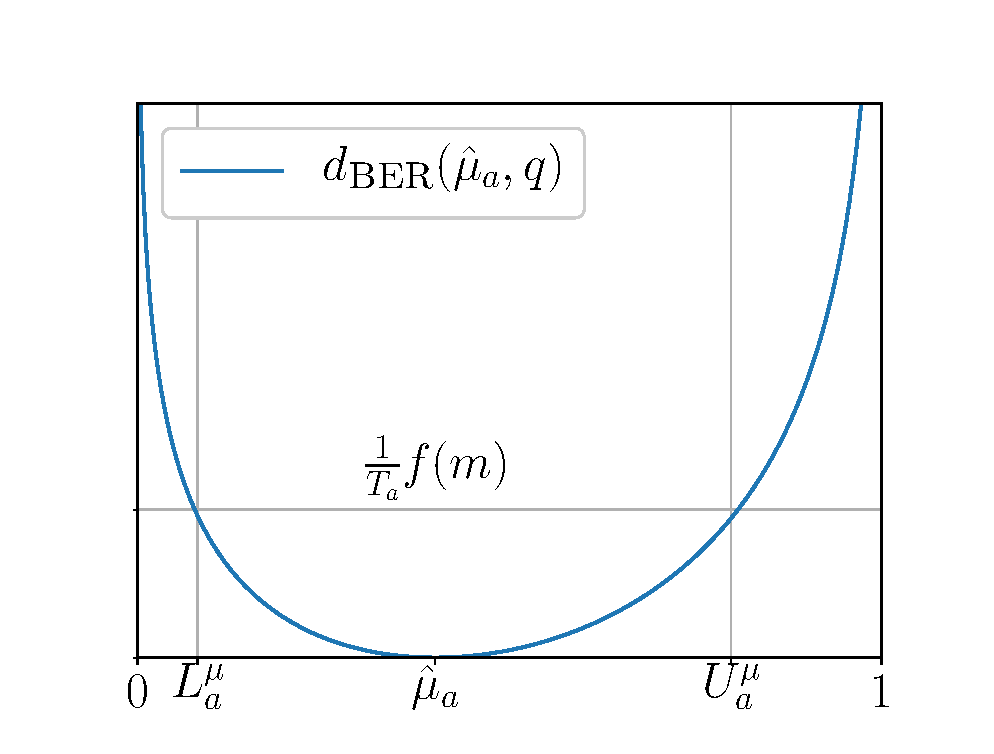
\includegraphics[width=0.6\textwidth]{../img/ukl}
\end{center}
\vspace{-1em}
Conversely,
\begin{itemize}
    \item \hlg{$U^{\mu}_a(m) \in I = [0, 1], \forall a$}. 
    \item The sequence $(U_{a_{1:t}}(m))_t$ is \hlg{non-increasing}
    \item $B_a(m) = U_a(m)$, the \emph{bound sharpening} step is \hlb{superfluous}.
\end{itemize}
\end{frame}

\begin{frame}{Sample complexity}

\begin{theorem}[Sample complexity]
\label{thm:regret}
\KLOLOP enjoys the same regret bounds as \OLOP. More precisely, \KLOLOP satisfies:
\begin{equation*}
    \expectedvalue r_n = \begin{cases}
      \tilde{\cO}\left(n^{-\frac{\log 1/\gamma}{\log \kappa'}}\right), & \text{if}\ \gamma\sqrt{\kappa'} > 1 \\
      \tilde{\cO}\left(n^{-\frac{1}{2}}\right), & \text{if}\ \gamma\sqrt{\kappa'} \leq 1
    \end{cases}
\end{equation*}
\end{theorem}
\end{frame}

\begin{frame}{Time complexity}
\begin{block}{Original \KLOLOP}
\emph{Compute $B_a(m-1)$ from \eqref{eq:Ba} \hlr{for all $a\in A^L$}}
\end{block}
\begin{block}{Lazy \KLOLOP}
\centering
\includesvg[width=0.6\textwidth]{../img/tree.svg}
\end{block}

\begin{property}[Time and memory complexity]
\begin{equation*}
    \frac{C(\texttt{Lazy KL-OLOP})}{C(\KLOLOP)} = \frac{\hleg{nK}}{\hler{K^{L}}}
\end{equation*}
\end{property}
\end{frame}

\begin{frame}{Experiments | Expanded Trees}
    \includesvg[width=\textwidth]{../img/tree_OPD}
\end{frame}

\begin{frame}{Experiments | Expanded Trees}
    \includesvg[width=\textwidth]{../img/tree_OLOP}
\end{frame}

\begin{frame}{Experiments | Expanded Trees}
    \includesvg[width=\textwidth]{../img/tree_KL-OLOP}
\end{frame}

\begin{frame}{Experiments | Highway}
    \includesvg[width=\textwidth]{../img/hw_return}
\end{frame}
\begin{frame}{Experiments | Gridworld}
    \includesvg[width=\textwidth]{../img/gw_return}
\end{frame}
\begin{frame}{Experiments | Stochastic Gridworld}
    \includesvg[width=\textwidth]{../img/gw_stoch_return}
\end{frame}

\begin{frame}
        \frametitle{References}
        \printbibliography
\end{frame}

\end{document}

